\section{Simulation investigations}
This section presents environment setup and later the results of simulation
investigations. It is important to describe simulation setup so that in the
future someone could repeat test or maybe extend the application.
\label{cha:Simulation_investugations}
\subsection{Simulation environment}
When it comes to classification problems there is always a problem of how to
divide available dataset into training and testing sets. One of the most common
approach to ensure proper classifier evaluation is cross validation (more
information about cross validation methods can be found in). There are
different types:
\begin{itemize}
    \item \textbf{holdout cross validation}- data set is separated into two sets, called the 
        training set and the testing set. Classifier is trained using the 
        training set only. Then the classifier is asked to predict the output 
        values for the data in the testing set. The advantage of this method is 
        that it is usually preferable to the residual method and takes no longer 
        to compute. However, its evaluation can have a high variance, because
        it depends heavily on which data points end up in the training set and 
        which end up in the test set
    \item \textbf{Leave-one-out cross validation}- the classifier is trained on all the
        available data except for one point and a prediction is made for that
        point and stored to compute the average error from all points. 
    \item \textbf{K-fold cross validation}- the data set is divided into $k$ subsets, 
        and the holdout method is repeated $k$ times. Each time, one of the $k$ subsets 
        is used as the test set and the other $k-1$ subsets are merged together to form 
        a training set.
\end{itemize}
In this thesis $4$-fold cross validation was used. To ensure that presented
results are reliable each test was repeated 10 times.
\label{cha:Simulation_environment}
\subsection{Simulation results}
\label{cha:Simulation_results}
\subsubsection{Impact of granulation step on rough sets efficiency}
\label{cha:Simulation_reaearch_1}
The aim of this test was to find out how the discretization of feature space
affect the classification accuracy. At first the number of intervals for each
attribute is the same and denoted as $K_l$, where $l \in (1, \ldots, d)$.
Results of the simulation are presented in table
\ref{tab:simulation_research_1} where the notation is as follows:
\begin{itemize}
    \item $G$- granulation step
    \item $O$- total number of correctly recognized objects
    \item $C/CD$- number of patterns for which a certain decision rules were
        used/number of correctly recognized patterns using these rules 
    \item $P/PD$- number of patterns for which a possible decision rules were
        activated/number of correctly classified objects using these rules
    \item $V$ number of patterns rejected from classification. There was no
        suitable rule or more rules have the same strength but different class
        label.
    \item $C^*, P^*, V^*$ - total number of certain, possible, void decision rules 
        respectively
\end{itemize}
In the experiment, for every feature the initial step of granulation was
changed from 4 to 18 while the factor of its increasing $\gamma$  was equal 
to one.

Analyzing the results of simulation presented in table \ref{tab:simulation_research_1}
one can see that the quality of the algorithm depends on the step of
granulation $G$ and better results are obtained rather for small $G$.
It can be concluded that decreasing the step of granulation causes that the number of 
decision formulas with the strength equal to zero is growing. The level of
discretization is correlated with the number of cells in which decision was 
certain or possible because of predominance of one class. In a situation with a small 
number of fields there were areas with the same number of object from both class, but 
small number of void cells. Decreasing the step of granulation results in more fields 
where decision was certain for one class, but at the same time it was noticeable that 
the number of areas without representative is increasing.

\begin{table}[H]
    \caption{Result of simulation for finding the dependency between
    granulation step and classification accuracy}
    \centering
    \begin{tabular}{|c|c|c|c|c|c|c|c|}
        \hline
        $G$ & $O$ & $C/CD$ & $P/PD$ & $V$ & $C^*$ & $P^*$ & $V^*$ \\ \hline \hline
        4&114&0/0&125/95&28/19&3&7&54 \\ \hline
        5&114&0/0&121/97&32/17&2&4&119 \\\hline
        6&114&3/1&65/51&85/62&5&8&203 \\ \hline
        7&115&0/0&91/74&62/41&3&6&334 \\ \hline
        8&113&2/1&24/17&127/95&8&9&495 \\ \hline
        9&114&4/4&59/48&90/62&6&7&716 \\ \hline
        10&112&36/25&38/32&79/55&12&13&975 \\ \hline
        11&112&5/2&30/23&118/87&7&9&1315 \\ \hline
        12&111&49/41&9/4&95/66&19&12&1697 \\ \hline
        13&109&0/0&13/9&140/100&17&12&2168 \\ \hline
        14&112&9/6&28/24&116/82&24&14&2706 \\ \hline
        15&105&30/25&17/4&106/76&27&13&3335 \\ \hline
        16&108&2/1&20/17&131/90&22&12&4062 \\ \hline
        17&100&3/1&38/24&112/75&24&17&4872 \\ \hline
        18&101&2/1&11/8&140/92&25&13&5794 \\ \hline
    \end{tabular}
    \label{tab:simulation_research_1}
\end{table}

\subsubsection{Impact of recursive modification of granulation step on rough sets
efficiency}
\label{cha:Simulation_reaearch_2}
In the previous section (\ref{cha:Simulation_reaearch_2}) it was shown that the
granulation step strongly affect the classification accuracy.
Greater $G$ implies that we have more certain or possible rule, but on the
other hand number of patterns without rule covering is increasing. A lot of
patterns are rejected because no proper rule is found. To improve that
situation algorithm for modification of decision rules is proposed. More
details are presented in section
\ref{cha:Algorithm_construction_rough_set_modification}, but generally when an
object is rejected from classification $G$ is decreased by $\epsilon=1$ until 
proper certain for possible solution is found. The same dataset was used as in
the previous one with the same algorithm settings. Results of classification
are presented in fig. \ref{fig:Simulation_research_2} for the basic rough
sets (blue line-BRS) and algorithm with modification of decision rules (orange
line-MRS).
\begin{figure}[H]
    \begin{center}
        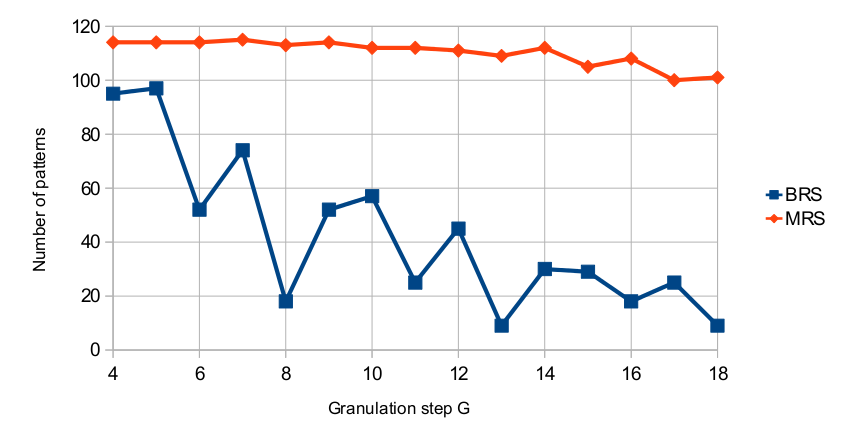
\includegraphics[width=\textwidth]{fig/rough_chart.png}
    \end{center}
    \caption{Comparison of Basic Rough sets algorithm with algorithm where
    modification of decision rules is introduced.}
    \label{fig:Simulation_research_2}
\end{figure}

Looking at fig. \ref{fig:Simulation_research_2} one can observer that
modification of granulation step $G$ increases the classification accuracy and
even if the granulation step is changed classification stays almost at the same
level while in the basic approach the greater $G$ implies worse results.
Additionally, it is visible that increasing granulation step is not the right
solution. Even if the number of certain or possible rules is greater the final
result is worse. Additionally, computational time is longer for greater $G$. In
this case the optimal $G$ would be 5, but for each problem $G$ should be chosen
independently because it must reflect how patterns are located in the feature
space.

The main two disadvantages of proposed rough sets algorithms are as follows:
\begin{itemize}
    \item it uses an arbitrary chosen step of granulation. Modification of
        decision rule improves classifier quality, but for the prize of
        computational time. 
    \item it uses all attributes for creation of decision rules. When the
        problem is complex decision rules are long and tangled. Additionally,
        some features are useless in classification, instead of valuable
        information bring noise to the system and deteriorate final results.
\end{itemize}

\subsubsection{Impact of number of membership functions on genetic fuzzy logic algorithm efficiency}
\label{cha:Simulation_reaearch_3}
In this section the results of fuzzy logic classifier simulation are presented.
The goal is to show that proposed algorithm construction is correct and gives
satisfactory results. 

At first, let remind what are the requirements for fuzzy logic classifier in
this thesis. As the input we have dataset without no expert knowledge of how to
appropriately divide feature space into fuzzy sets, how many membership
functions we need. The goal is to minimal rule set with the possible highest
classification accuracy. 

As the first step let present how fuzzy logic classifier deals with pattern
recognition and what is the minimal rule set for exemplary dataset which is
iris dataset with four attributes. At the beginning each feature was divided
into 14 membership functions in the same way as presented in fig. \ref{fig:fuzzy_example}
The final rule set which was able to classify 32 out of 34 testing pattern is
presented in fig. \ref{fig:fuzzy_result}:
\begin{figure}[H]
    \begin{center}
        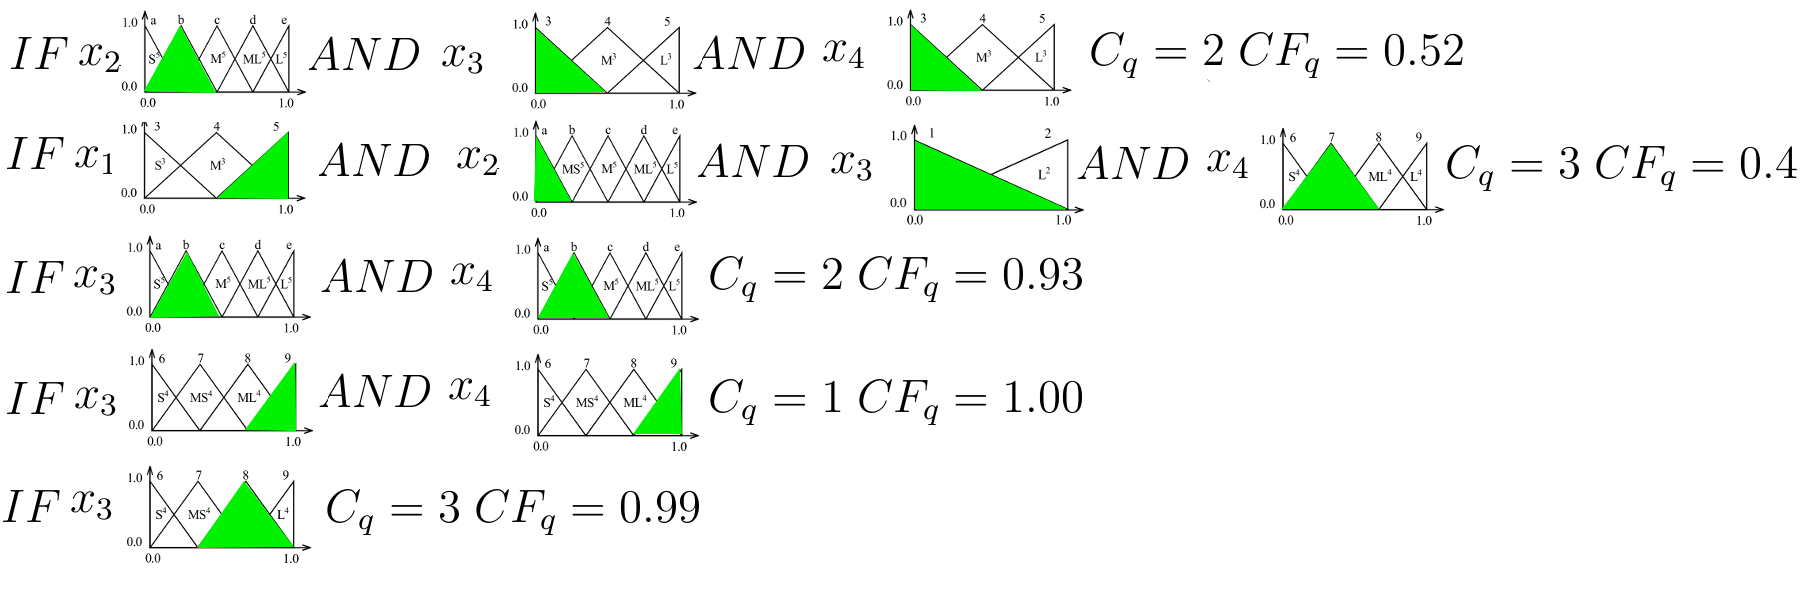
\includegraphics[width=\textwidth]{fig/fuzzy_result.png}
    \end{center}
    \caption{Example of rule set generated for Iris dataset}
    \label{fig:fuzzy_result}
\end{figure}
Analyzing figure \ref{fig:fuzzy_result} it is visible that some attributes were
omitted from classification, but the results of classification are quite
satisfactory. Additionally, only five rules were needed for correct pattern
recognition.

The goal of the second part of this test was to check how the number of initial
membership functions affects the final result of classification. There is a
question if it is better to use many small membership functions (for example 14
functions such as presented in fig. \ref{fig:fuzzy_example}}) or only few
functions with greater area coverage. In the first case the solution space is 
much greater than in the second approach so many rules must be created to obtain 
reliable results. Additionally, in most recognition problems we do not need so precise
feature partitions because it can happen that for many created regions we
cannot find proper representatives in the training set. 
Parameters for genetic algorithms are the same as presented
in table \ref{tab:fuzzy_genetic_parameters}. In each simulation the level of
partitions $k$ was changed from $7$ to $2$. Few words of explanation should be
written about how $k$ determines the number of membership functions $MF$ for each
attribute. This number is described by eq. (\ref{eq:fuzzy_function_number})
\begin{equation}
    MF = \sum\limits_1^k (n + 1) + 1
    \label{eq:fuzzy_function_number}
\end{equation}

\begin{figure}[H]
    \begin{center}
        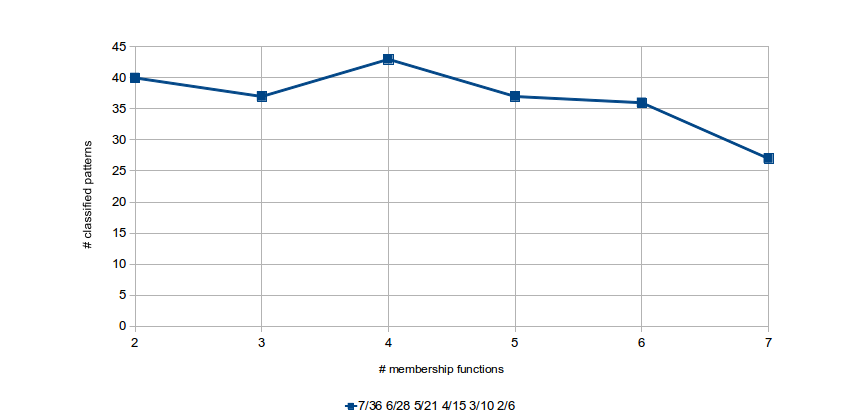
\includegraphics[width=\textwidth]{fig/fuzzy_functions.png}
    \end{center}
    \caption{Impact of initial number of membership functions $MF$ per attribute on
    the final fuzzy classification rate}
    \label{fig:fuzzy_functions}
\end{figure}
Looking at the fig. \ref{fig:fuzzy_functions} one can conclude that it is not
worth increasing the number of membership functions ($MF$) per attribute
because for greater $MF$ algorithm obtained worse results in case of
classification accuracy. From conducted simulations it was concluded that the
optimal $k$ value is 4. If not implicitly stated, $k=4$ will be used in next
tests.

\subsubsection{Impact of granulation step $G$ on genetic rough sets algorithm efficiency}
\label{cha:Simulation_reaearch_4}
The goal of this test is to check which approach is better:
\begin{enumerate}
    \item use the same granulation step $G$ for each attribute and additionally
        take all feature into classification
    \item use different partition for each attribute independently and try to
        remove some features treating them as a noise.
\end{enumerate}
The first approach is simulated by algorithm with modification of decision
rules (see section
\ref{cha:Algorithm_construction_rough_set_modification}), while the second
is genetic rough sets algorithm (described in section \ref{cha:Multistage}),
where the notation is as follows:
\begin{itemize}
    \item $A$ number of attributes describing pattern in dataset
    \item $O$ number of patterns for classification
    \item $RSR$ number of objects correctly recognized by basic rough sets
        algorithm
    \item $RSMR$ number of patterns correctly recognized by rough sets
        algorithm with modification of decision rules
    \item $GRR$ number of objects correctly recognized by genetic rough sets
        algorithm
    \item $AU$ number of features used by genetic rough sets algorithm for
        classification.
\end{itemize}

Results of simulation are presented in table \ref{tab:genetic_rough_results}.
Parameters for genetic rough sets algorithm were the same as presented in table
\ref{tab:rough_genetic_parameters} and for the first rough sets algorithm
granulation step $G$ was equal to 5 and for algorithm with modification of
decision rules starting granulation value was $7$.
\begin{table}[H]
    \centering
    \begin{tabular}{|c|c|c|c|c|c|c|}
        \hline
        Dataset & $A$ & $O$ & $RSR$ & $RSMR$ & $GRR$ & $AU$\\ 
        \hline \hline
        haberman& 3&	76&	49&	58&	61 & 2 \\ \hline
        iris&	4&	39&	32&	38&	39 & 2\\ \hline
        bupa&  	6&	86&	28&	53&	57 & 3\\ \hline 
        pima&   8&	192&	69&	126& 155 & 5 \\ \hline
        wine& 13&	45&	0&	15&	44 & 2\\ \hline
    \end{tabular}
    \caption{Accuracy of classification for genetic rough sets and basic rough
    sets algorithms for different datasets}
    \label{tab:genetic_rough_results}
\end{table}
From table \ref{tab:genetic_rough_results} one can conclude that genetic rough
sets algorithm obtains better results than other algorithms, especially it is
visible for more complex problems such as wine or pima datasets. Additionally,
let analyze the last column $AU$. It determines how many attributes are used in
genetic rough sets algorithm for classification. It is noticeable that some
features are useless and genetic rough sets algorithm is able to find
valuable attributes. Another thing to reconsider is how the complexity of the
problem affects algorithm classification accuracy. Basic rough sets algorithm
tackles quite well with simple problems, for example iris or haberman datasets,
but when the number of attributes is greater than $4$ algorithm efficiency
decreases, while genetic rough sets is not affected by this problem and can
deal with complex datasets.


\subsubsection{Comparison of hybrid classifier with other classifiers}
\label{cha:Simulation_reaearch_5}
In this section results for hybrid classifier are presented. The accuracy of
classification is compared with other classifiers trained and tested with the
same datasets. The main goal of this simulation was to check if proposed
solution can compete with other classifiers. As the source of reference
different types of classifiers were chosen to ensure the greatest diversity:
\begin{itemize}
    \item LDAC classifier (Linear Discriminant classifier)- The linear
        discriminant analysis method consists of searching, some linear
        combinations of selected variables, which provide the best separation between the
        considered classes. These different combinations are called
        discriminant functions (see example in fig. \ref{fig:ldac_example})
        \begin{figure}[H]
            \begin{center}
                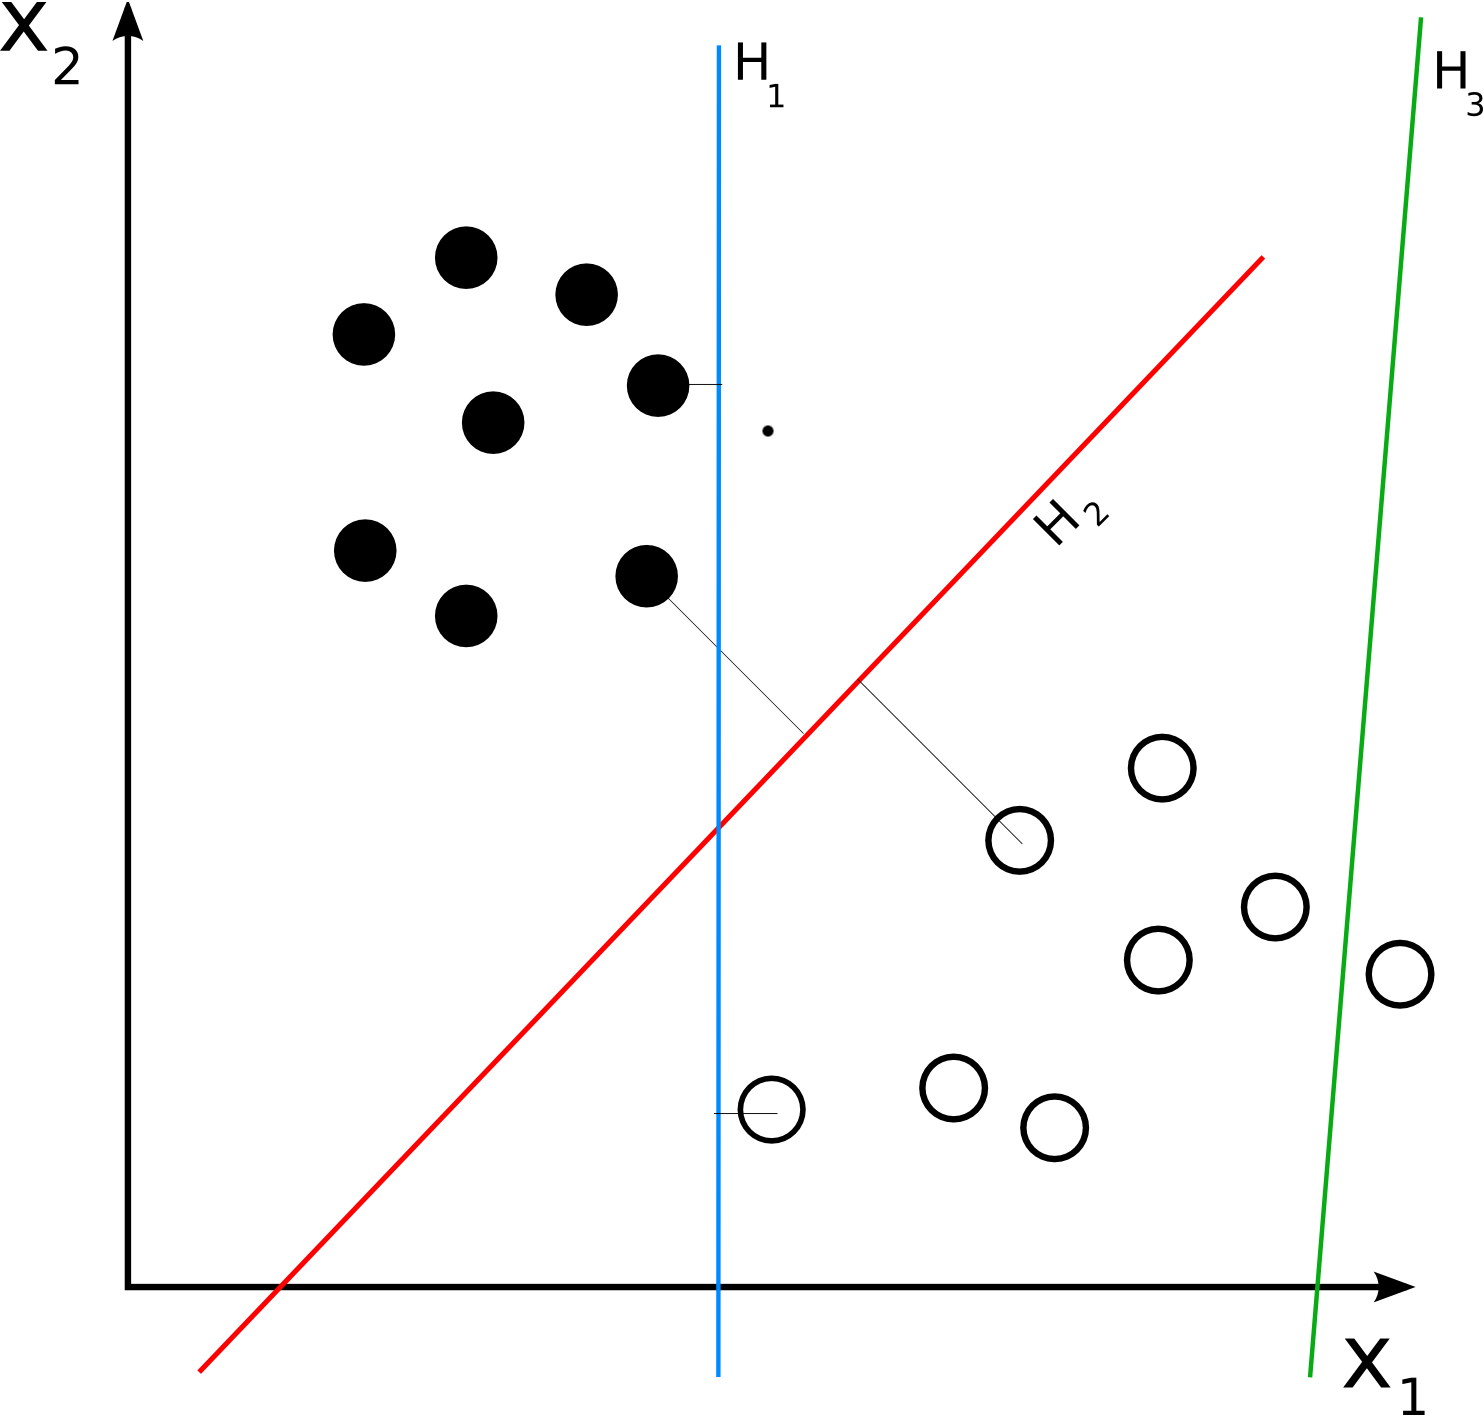
\includegraphics[width=0.6\textwidth, height=0.5\textwidth]{fig/ldac.png}
            \end{center}
            \caption{Example of linear discriminant classifier for 2-dimensional problem}
            \label{fig:ldac_example}
        \end{figure}
    \item 3-KNN Classifier- it is one of the simplest approach in the pattern
        recognition, it classifies objects based on closest training examples
        in the feature space.
    \item Gini index classifier- it is an example of decision tree algorithm
        where the decision is represented in case of decision rules.  Decision
        node specifies a test on a single attribute, leaf node indicates the
        value of the target attribute, arc/edge splits of one attribute and
        path indicated the disjunction of test to make the final decision. 
        Decision trees classify instances or examples by starting at the root 
        of the tree and moving through it until a leaf node is reached.
    \item Maximum likelihood classifier- this classifier is commonly used in
        image recognition tasks. It assigns a pixel to a class on the basis of
        its probability of belonging to a class whose mean and covariance are
        modelled as forming a normal distribution in multidimensional feature
        space.
    \item Svm classifier- it is non-probabilistic linear classifier which 
        deals with finding an optimal linear hyperplanes for class separation.
\end{itemize}
Results of simulation are presented in table \ref{tab:final_comparison}, where
$O$ determines the number of patterns for classification. Last row in table
shows results for hybrid classifier described in section
\ref{cha:Multistage_rough_fuzzy}. Numbers in bold font indicates which
classifier obtained the best result for a particular dataset.

\begin{table}[H]
    \caption{Comparison of hybrid rough fuzzy classifier with other common
    classifiers}
    \centering
    \begin{tabular}{|c|c|c|c|c|c|c|c|}
        \hline
        Algorithm&iris&bupa&pima&haberman&wine&wdbc&thyroid \\ \hline \hline
        $O$&39&86&192&76&45 & 142 & 55\\ \hline
        LDAC&38&62&146&58&44& \textbf{138} &51 \\ \hline
        3-KNN&38&56&131&56&32 & 133 &52 \\ \hline
        Gini Index&38&56&123&58&41& 131 &53 \\ \hline
        Max likelyhood&38&51&145&58&45 & 135 &55\\ \hline 
        Svm&26&\textbf{63}&141&56&43& 133 & 53\\ \hline \hline
        \textbf{Hybrid}&\textbf{39}&59&\textbf{155}&\textbf{61}&\textbf{45}&
        135 & \textbf{55}\\ \hline
    \end{tabular}
    \label{tab:final_comparison}
\end{table}

From table \ref{tab:final_comparison} one can conclude that hybrid classifier
obtains quite good results comparing with other classifiers. From seven
datasets five times it was the best. In other cases results are comparable.
What is more important hybrid classifier is able to classify pattern with
reduced number of attributes. In this case created decision rules are simpler
and more readable for user. This is especially important in medicine where
physician is provided with decision rules and basing on them makes the final
diagnosis. Another thing to reconsider is the stability of proposed classifier.
It uses genetic algorithm for rule construction, so taking into account its
random nature hybrid classifier can be unstable, but simulations show that this
is not a problem. Appropriate number of generations for genetic algorithm
assures proper convergence and as the consequence hybrid classifier is stable. 
